\documentclass[final]{fhnwreport}       %[mode] = draft or final
                                        %{class} = fhnwreport, article, 
                                        %          report, book, beamer, standalone
\input{header}			                %loads all packages, definitions and settings												
\title{\Huge{\textbf{EMV-Projektbericht}}\\}          %Project Title
\author{\huge{Versuchsname}}          %Document Type => Technical Report, ...
\date{Windisch, \today}             %Place and Date


\begin{document}

%%---TITLEPAGE---------------------------------------------------------------------------
\selectlanguage{ngerman}                %ngerman or english
\maketitle
%\vspace*{-1cm}
\vspace*{-0.5cm}						    %compensates the space after the date line.
\vfill
\begin{figure}[H]
\centering
\includegraphics[width=\linewidth]{Titelbild.jpg}
\end{figure}
\vfill

{
\renewcommand\arraystretch{2}
\begin{center}
\begin{tabular}{>{\bf}p{4cm} l}
Hochschule                 &    Hochschule für Technik - FHNW\\
Studiengang                &    Elektro- und Informationstechnik\\
Autor/-en  		           & 	Mischa Knupfer, Simon Hasler\\
Dozent                   &    Pascal Schleuniger\\
Modul               &    EMV\\
Version                    &    1.0 %Normally not used!
\end{tabular}
\end{center}
}

\clearpage
			
%%---ABSTRACT----------------------------------------------------------------------------
\selectlanguage{english}				%ngerman or english
\thispagestyle{empty}
%\begin{abstract}
\noindent


\end{abstract}	

%%---TABLE OF CONTENTS-------------------------------------------------------------------
\pagenumbering{Roman}		
\selectlanguage{ngerman}				%ngerman or english
\tableofcontents
\clearpage

%%---TEXT--------------------------------------------------------------------------------
\pagenumbering{arabic}
\section{Einleitung}

%Auftrag
%Was wird gemacht?
%Wie ist der Bericht aufgebaut?
\section{Schaltung}
\label{sec:Schaltung}

%Schaltung zeigen
%Funktionsweise der Schaltung
%Welche Tests sinnvoll und warum

In der Bachelor-Thesis von Simon Hasler ist eine Teilschaltung implementiert, welche den Strom eines Asynchronmotors misst. Diese Schaltung wurde von den Autoren ausgewählt, um im Modul EMV Tests durchführen zu können. Damit die Schaltung bei den Tests sicher nicht kaputt geht, sollte diese nachgebaut werden. Leider wurde bekannt, dass diese Teilschaltung, generiert von einer anderen, externen Schule, nicht funktionstüchtig ist. Aus diesem Grund haben die Autoren eine eigene Schaltung zur Strommessung mit an der Fachhochschule zur Verfügung stehenden Mitteln zusammengestellt. Bei der Schaltung handelt es sich um eine Strommessung über einen Widerstand (Shunt) mit Tiefpassfilterung und einem Operationsverstärker, zu sehen in Abbildung \ref{fig:SchaltungDraw}.\\

\begin{minipage}[b][6cm][t]{1\textwidth}
\centering
\includegraphics[angle=0,width=0.75\textwidth]{graphics/SchaltungDraw.jpg}
\captionof{figure}{Schema der entworfenen Schaltung.}
\label{fig:SchaltungDraw}
\end{minipage}
\vspace*{0.25cm}

In Abbildung \ref{fig:SchaltungDraw} ist zu sehen, dass von Links der zu messende Strom in die Schaltung hinein und durch den Shunt (R1) strömt. Ein Tiefpassfilter (R2 parallel zu C1) schützt die nachfolgende Schaltung vor Schäden durch hohe Frequenzen. Der Operationsverstärker (U1) dient als nichtinvertierender Verstärker mit einem Verstärkungsfaktor von $1+\dfrac{R3}{R4}$. Die Ausgangsspannung, welche im Verhältnis zum zu messenden Strom ist, wird an einen Mikrocontroller zur Datenverarbeitung weiteregeben (bzw. erst auf einen ADC). Der Operationsverstärker benötigt zudem eine Spannungsversorgung von +5V.\\

Das Schema wird umgesetzt mit Bauteilen, welche direkt an der Fachhochschule bezogen werden können. Ebenfalls wird nicht extra ein Print hergestellt, sondern eine Lochrasterplatine verwendet, auf welcher die Schaltung gelötet wird. Die Schaltung sieht umgesetzt aus wie in Abbildung \ref{fig:Schaltung1} aus.

\begin{minipage}[b][6cm][t]{1\textwidth}
\centering
\includegraphics[angle=0,width=0.75\textwidth]{graphics/Schaltung1.jpg}
\captionof{figure}{Die realisierte entworfene Schaltung.}
\label{fig:Schaltung1}
\end{minipage}
\vspace*{4cm}

In Abbildung \ref{fig:Schaltung1} sind die Anschlüsse für eine Stromquelle (1), für den Ausgang zur MCU bzw. zum Oszilloskop (3) und für die Speisespannung des Operationsverstärkers (2) zu sehen. Die Schaltung selbst, wie in Abbildung \ref{fig:SchaltungDraw} gezeichnet, ist ebenfalls zu sehen (4). Ausserdem sind die Schutzelemente gegen die ausgewählten EMV-Störungen hier schon implementiert (5), was jedoch erst in Kapitel \ref{sec:Schutz} näher besprochen wird.\\

Damit sichergestellt ist, dass die Schaltung ihre Aufgabe erfüllt, muss dies getestet werden. Dafür wird der Ausgang an ein Oszilloskop angeschlossen, der Operationsverstärker mit einer Spannungsquelle gespiesen (5V) und am Eingang eine Stromquelle angeschlossen. Nun sollen für verschiedene Ströme auch verschiedene Spannungslevel auftreten. Die Auswertung ist zu sehen in Abbildung \ref{fig:Schaltungstest}.\\

\begin{minipage}[b][6cm][t]{1\textwidth}
\centering
\includegraphics[angle=0,width=0.75\textwidth]{graphics/Schaltungstest.jpg}
\captionof{figure}{Das Ergebnis des Funktionstest, geplottet mit QtiPlot.}
\label{fig:Schaltungstest}
\end{minipage}
\vspace*{4cm}

Abbildung \ref{fig:Schaltungstest} zeigt die am Oszilloskop gemessene Spannung für verschiedene Eingangsströme. Es fällt ein linearer Zusammenhang auf, wobei es zu kleineren Abweichung (Messfehler, Ablesefehler...) kommt. Die Schaltung gibt also für jeden Eingangsstrom einen anderen Spannungspegel aus, weshalb gesagt werden kann, dass die Schaltung funktioniert.\\

Die Schaltung wurde aufgebaut und auf ihre Funktionalität getestet. Als nächstes folgen die ausgewählten EMV-Testarten und deren Normen, auf diese hin die Schaltung getestet wird.\\



\section{Testarten und Normen}
\label{sec:TestUndNorm}
%Welche Testarten gibt es?
%Welche sind sinnvoll bei unserer Schaltung?
\section{Schutzelemente}

%Was für Schutzelemente gibt es?
%Wie kann die Schaltung geschützt werden?

\section{Testaufbau}

%Aufzeigen was wie getestet wird und mit welchem Aufbau
\section{Testprotokoll: Burst}
\label{sec:Test:Burst}


\section{Testprotokoll: Surge}
\label{sec:Test:Surge}
Wie in Kapitel \ref{sec:TestUndNorm} erwähnt, werden Surge-Tests zurchgeführt. Zur Auswahl stehen gemäss Kapitel \ref{sec:TestUndNorm} vier verschiedene Normprogramme. Es wurden das erste (Level 1) und das letzte (Level 4) Normprogramm durchgeführt, deren Ergebnisse werden nachfolgend dokumentiert. Der Testaufbau und die verwendeten Geräte werden in Kapitel \ref{sec:Testaufbau} erläutert.\\[0.25cm]
Die Auswirkungen der Tests wurden mit einem Oszilloskop gemessen. Nachfolgend werden die Abbildungen davon aufgezeigt und kurz erläutert.\\[0.5cm]
\begin{minipage}[b][10cm][t]{1\textwidth}
\centering
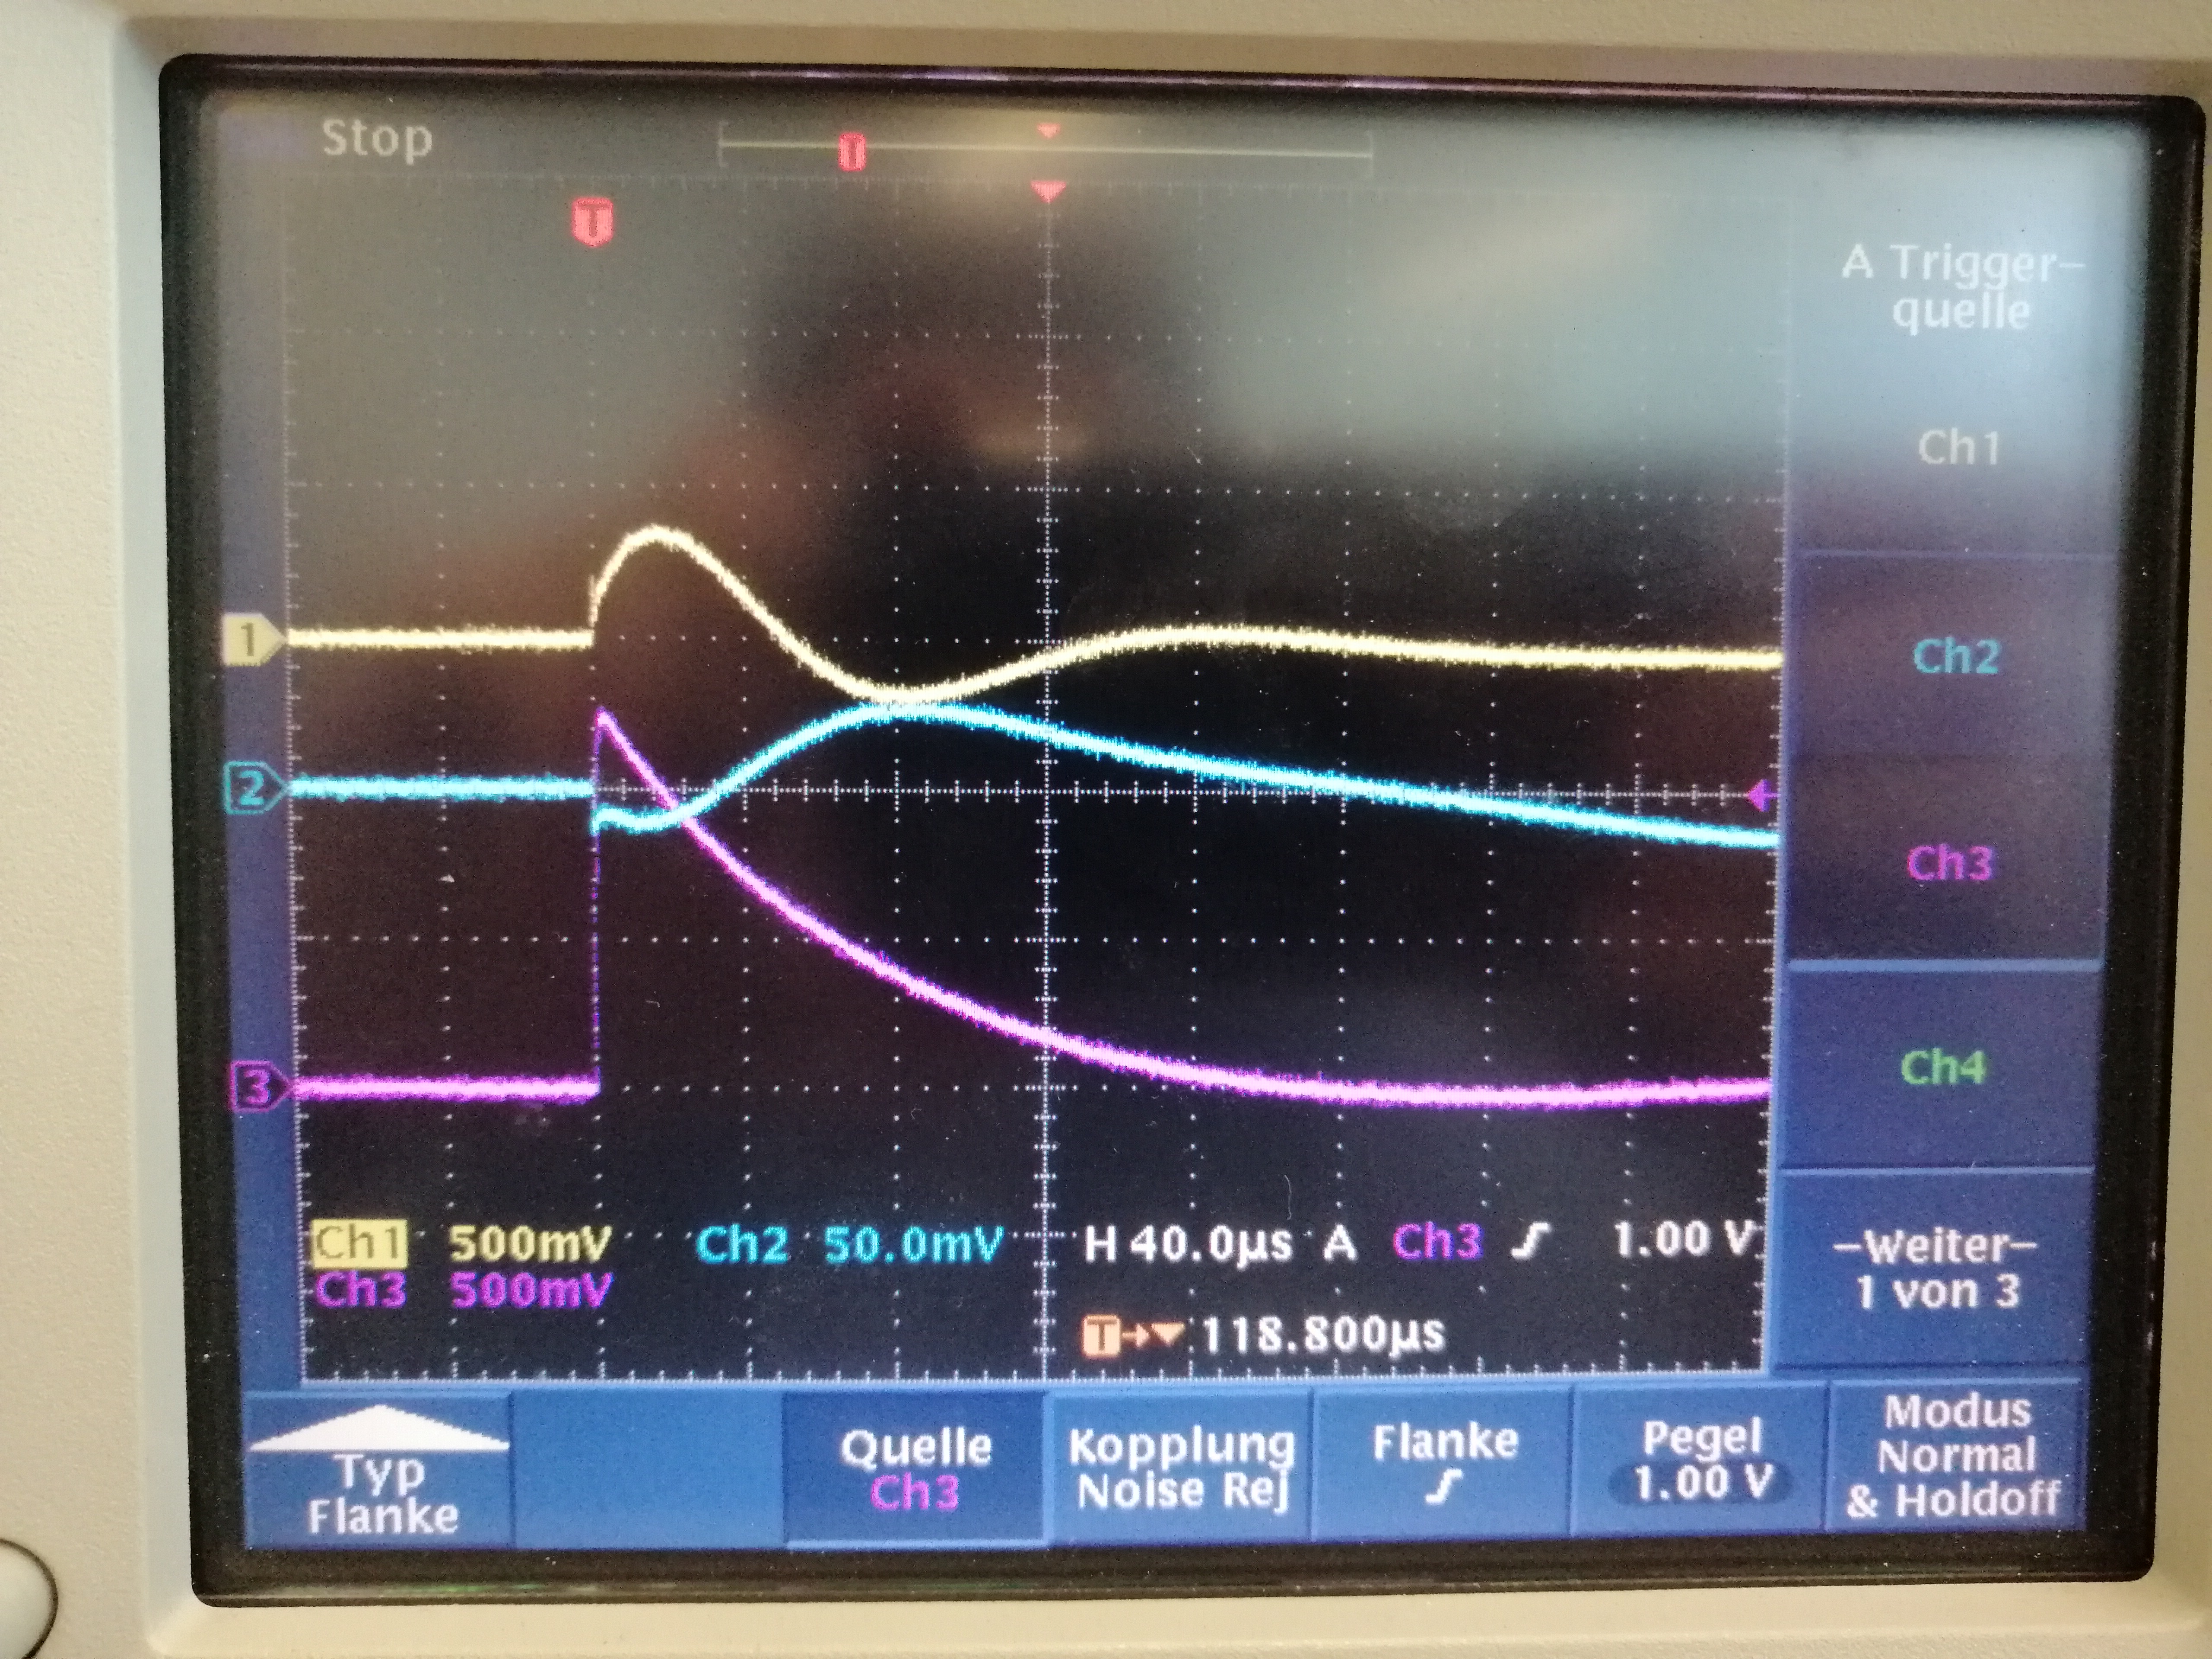
\includegraphics[angle=0,width=0.75\textwidth]{graphics/Surge1.jpg}
\captionof{figure}{Signalmessung während Surge-Test, Level 1, positive Polarität.}
\label{fig:Surge1}
\end{minipage}
Abbildung \ref{fig:Surge1} zeigt die verschiedenen Messsignale. Die Stossspannung des Surge-Tests (Lila) ist deutlich zu sehen mit einer steilen Flanke und einem Abklingen über 200$\mu$s. Der zur Stossspannung zugehöriger Strom (Blau) ist ebenfalls zu sehen mit einem kleinen, steilen Abfall, gefolgt von einer Erhöhung welche sich dann wieder senkt. Das Messsignal (Gelb) zeigt eine Überhöhung mit gefolgtem Einschwingen über ebenfalls etwa 200$\mu$s.\\[0.5cm]
\begin{minipage}[b][10cm][t]{1\textwidth}
\centering
\includegraphics[angle=0,width=0.75\textwidth]{graphics/Surge2.jpg}
\captionof{figure}{Signalmessung während Surge-Test, Level 1, negative Polarität.}
\label{fig:Surge2}
\end{minipage}
Abbildung \ref{fig:Surge2} zeigt das gespiegelte Verhalten von Abildung \ref{fig:Surge1}.\\[0.5cm]
\begin{minipage}[b][10cm][t]{1\textwidth}
\centering
\includegraphics[angle=0,width=0.75\textwidth]{graphics/Surge3.jpg}
\captionof{figure}{Signalmessung während Surge-Test, Level 4, positive Polarität.}
\label{fig:Surge3}
\end{minipage}
Abbildung \ref{fig:Surge3} zeigt die verschiedenen Messsignale. Die Stossspannung des Surge-Tests (Lila) ist deutlich zu sehen mit einer steilen Flanke und einem Abklingen über 240$\mu$s. Der zur Stossspannung zugehöriger Strom (Blau) ist ebenfalls zu sehen mit einem kleinen, steilen Abfall, gefolgt von einer Erhöhung welche sich dann wieder senkt. Das Messsignal (Gelb) zeigt eine Überhöhung mit gefolgtem Einschwingen über ebenfalls etwa 240$\mu$s.\\[0.5cm]
\begin{minipage}[b][10cm][t]{1\textwidth}
\centering
\includegraphics[angle=0,width=0.75\textwidth]{graphics/Surge4.jpg}
\captionof{figure}{Signalmessung während Surge-Test, Level 4, negative Polarität.}
\label{fig:Surge4}
\end{minipage}
Abbildung \ref{fig:Surge4} zeigt das gespiegelte Verhalten von Abildung \ref{fig:Surge3}.\\[0.5cm]
\begin{tabular}{|l|l|p{5cm}|p{5cm}|}
\hline 
\rule[-1ex]{0pt}{2.5ex} Prüfspannung & Prüflevel & Anzahl Surges pro Polarität & Auswirkung \\ 
\hline 
\rule[-1ex]{0pt}{2.5ex} 500 V & 1 & Bis mindestens 1 Surge mit dem Oszilloskop gut eingefangen werden konnte & Verlust der Messfähigkeit bei aktivem Surge. Wieder funktionsfähig unmittelbar nach dem Surge. \\ 
\hline 
\rule[-1ex]{0pt}{2.5ex} 4000 V & 4 & Bis mindestens 1 Surge mit dem Oszilloskop gut eingefangen werden konnte & Verlust der Messfähigkeit bei aktivem Surge. Wieder funktionsfähig unmittelbar nach dem Surge. \\ 
\hline 
\end{tabular} 
\captionof{table}{Prüfungsergebnis Surge-Tests.}
\label{tab:SurgeErgebnis}
\vspace*{0.25cm}
Tabelle \ref{tab:SurgeErgebnis} listet die Ergebnisse der durchgeführten Surge-Normprogramme auf. Es ist zu erkennen, dass bei jedem Surge-Test die gleichen Auswirkungen zu sehen waren. Die Gesamtauswertung der Tests wird in einem separaten Kapitel (Kapitel \ref{sec:Auswertung}) behandelt.\\

%\include{sections/ESD}
\section{Testauswertung}
\label{sec:Auswertung}

\section{Schluss}


%Was wurde gemacht?
%Was sind die Resultate?
%Was haben wir gelernt?
%Was kann besser gemacht werden?



%%---BIBLIOGRAPHY------------------------------------------------------------------------
{\sloppypar
\printbibliography[heading=bibintoc]
\label{sec:lit}
%\selectlanguage{english}				%ngerman or english
%\printbibliography[heading=bibintoc]
}

%%---APPENDIX----------------------------------------------------------------------------
\begin{appendix}
%Anhänge

\end{appendix}

%%---NOTES for DEBUG---------------------------------------------------------------------
\ifdraft{%Do this only if mode=draft
%%requires \usepackage{todonotes})
\newpage
\listoftodos[\section{Todo-Notes}]
\clearpage
}
{%Do this only if mode=final
}
\end{document}
